
\subsection{Muon reconstruction}

Muons are reconstructed with information from the inner detector (ID),
the muon spectrometer (MS), and to a lesser extent, the
calorimeters. In the MS, track segments are first identified in each
layer, and then combined in a track fit (more information to be
consistent with other sections). Muon candidate tracks are
reconstructed in the ID according to the procedure in
section~\ref{chap:reco:sec:tracks}.

\subsection{Muon identification}

There are four muon identification schemes that take advantage of the
information from the different detector subsystems~\cite{bib:Aad:2014rra}. Stand-alone (SA)
muons are reconstructed with tracks from the MS only. The track of the
muon candidate is extrapolated back to the distance of closest
approach with the beam line, accounting for energy lost in the
calorimeter. These muons are required to have hits in at least two MS
layers. Because the MS extends to $|\eta| < 2.7$, SA muons recover
acceptance for muons which fall beyond the ID tracking volume $|\eta|
< 2.5$. For combined (CB) muons, muon tracks are independently
reconstructed in both the ID and the MS and then
combined. Segment-tagged (ST) muons are those for which there exists
an ID track which, when extrapolated to the MS, corresponds to a track
segment in a MDT or CSC layer. This type recovers acceptance
associated with muons that only traverse a single MS layer due to the
limited coverage of the MS or because the muon \pt~is low. Finally,
for calorimeter tagged (CaloTag) muons, an ID track is associated with
an energy deposit in the calorimeter that is consistent with a
minimum-ionizing particle. 

For the analysis presented in this thesis, only CB muons are used. The
combination of the ID and MS tracks is done by statistically combining
the two tracks with their respective parameters and covariance
matrices. Starting with a set of ID tracks and a set of MS tracks,
MS-ID track pairs are matched in $\eta$ and $\phi$, and the MS-ID track
pair with the smallest combined $\chi^2$ is retained as a CB muon. The
constituent tracks are then removed from the set and the next iteration
proceeds until there are no more candidate tracks. To suppress
background, the ID tracks that are used require at least 1 pixel hit,
5 SCT hits, and at least 9 TRT hits in the region with full TRT
coverage. Moreover, tracks can only have a maximum of 2 active pixel or
SCT sensors without hits along the track trajectory.

As with electrons, it is crucial to know the reconstruction and
identification efficiencies for muons of various transverse momentum
and pseudorapidity. The efficiencies are measured with the
tag-and-probe method on \Zmm~events in which two oppositely charged
and isolated muons with $\pt>25 (10) \gev$ have dilepton invariant
mass that falls within 10 \gev~of $m_Z$. Tag muons are required to
satisfy CB requirements, and the efficiency of identifying a probe CB
muon is measured as a function of \pt~and $\eta$, as shown in
figure~\ref{chap:reconstruction:fig:muon_tp}. The efficiency for CB
muons is between 95\% and 100\% across most of the $\eta$ range,
although it falls to zero at $|\eta|<0.1$, due to a gap in the MS
coverage. In general, the efficiency as measured in data agrees quite
well with that of simulation, with the exception of the barrel-endcap
transition region ($0.9<\eta<1.3$), where there are imperfections in the
modeling of the detector. (need to say something about the pT plot in
the figure).

\begin{figure}[h!]
    \centering
    \subfigure{
    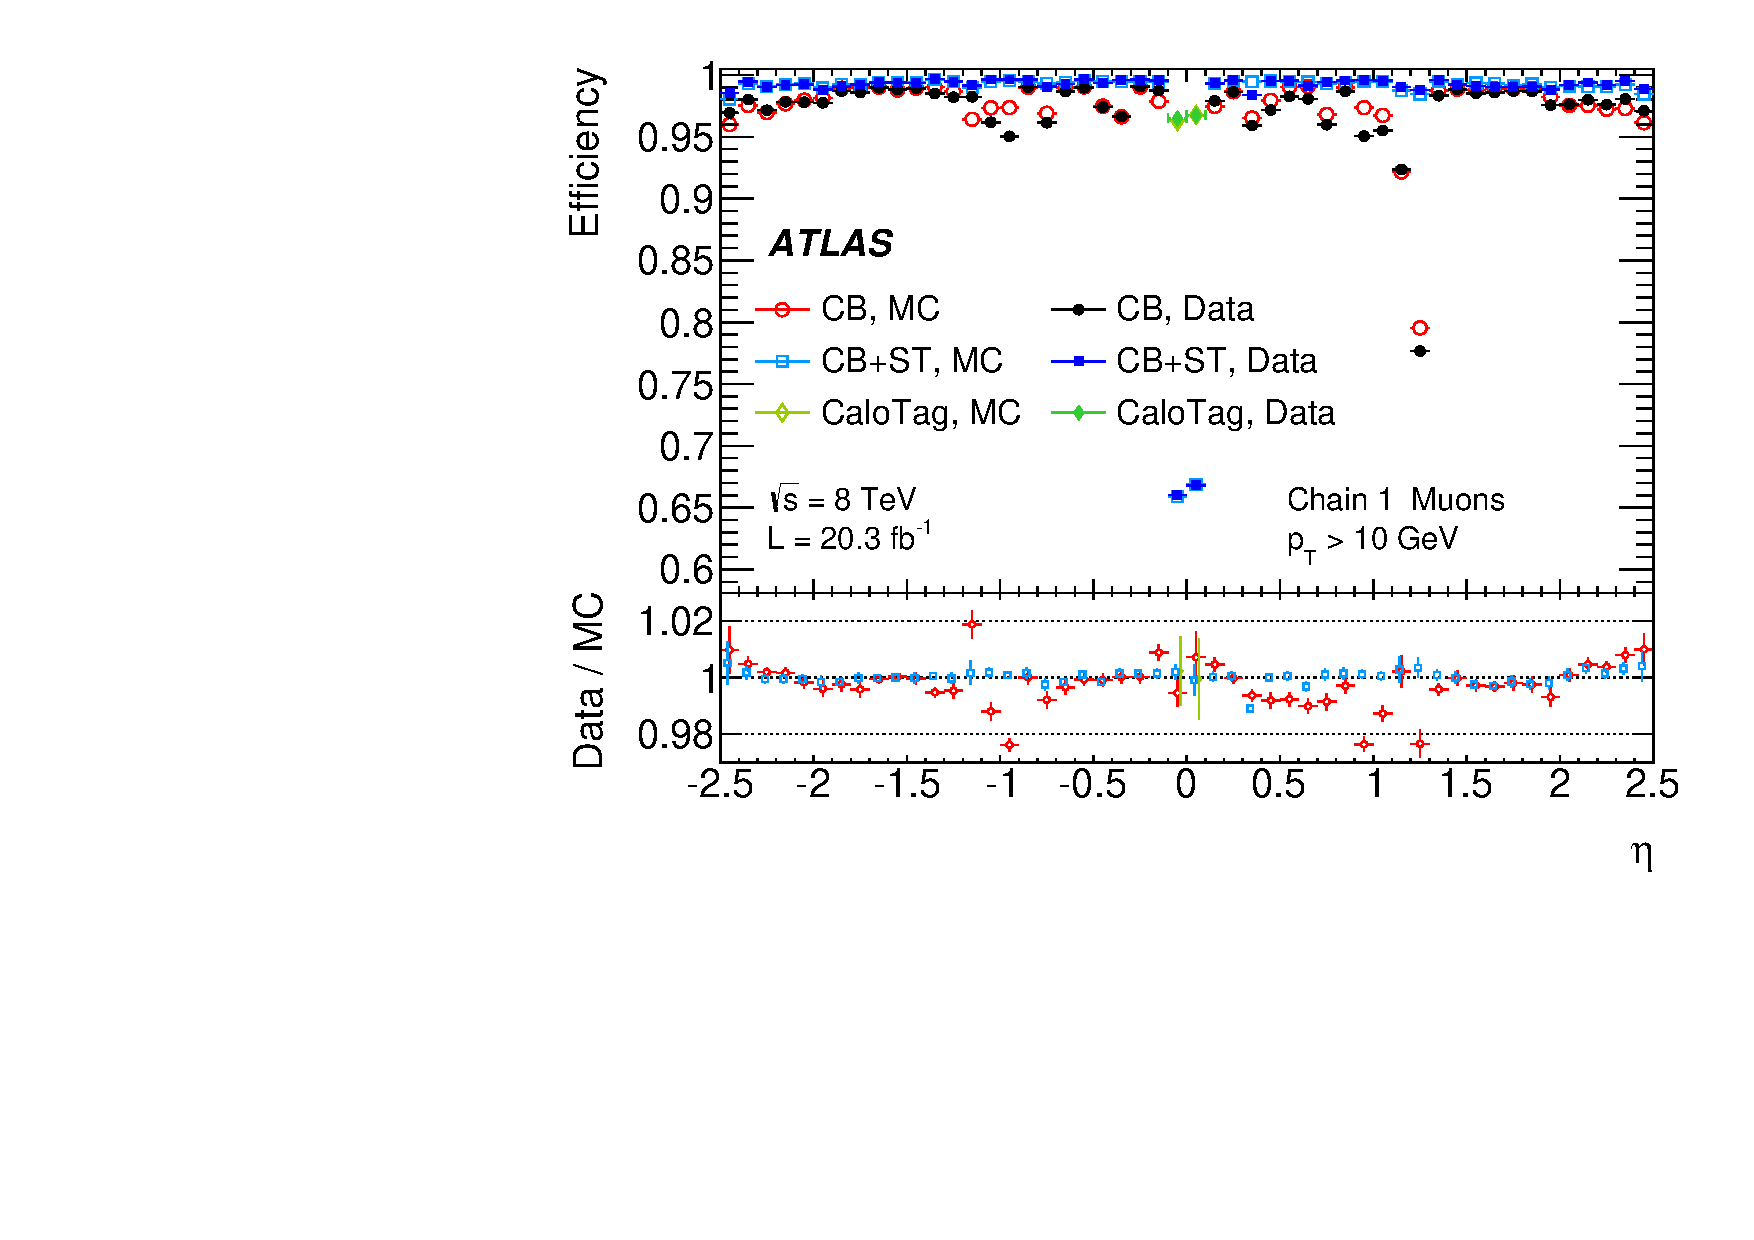
\includegraphics[width=0.4\textwidth]{fig/reconstruction/muon_TP_eta.pdf}
    \label{chap:reconstruction:fig:muon_tp_eta}
    }
    \subfigure{
    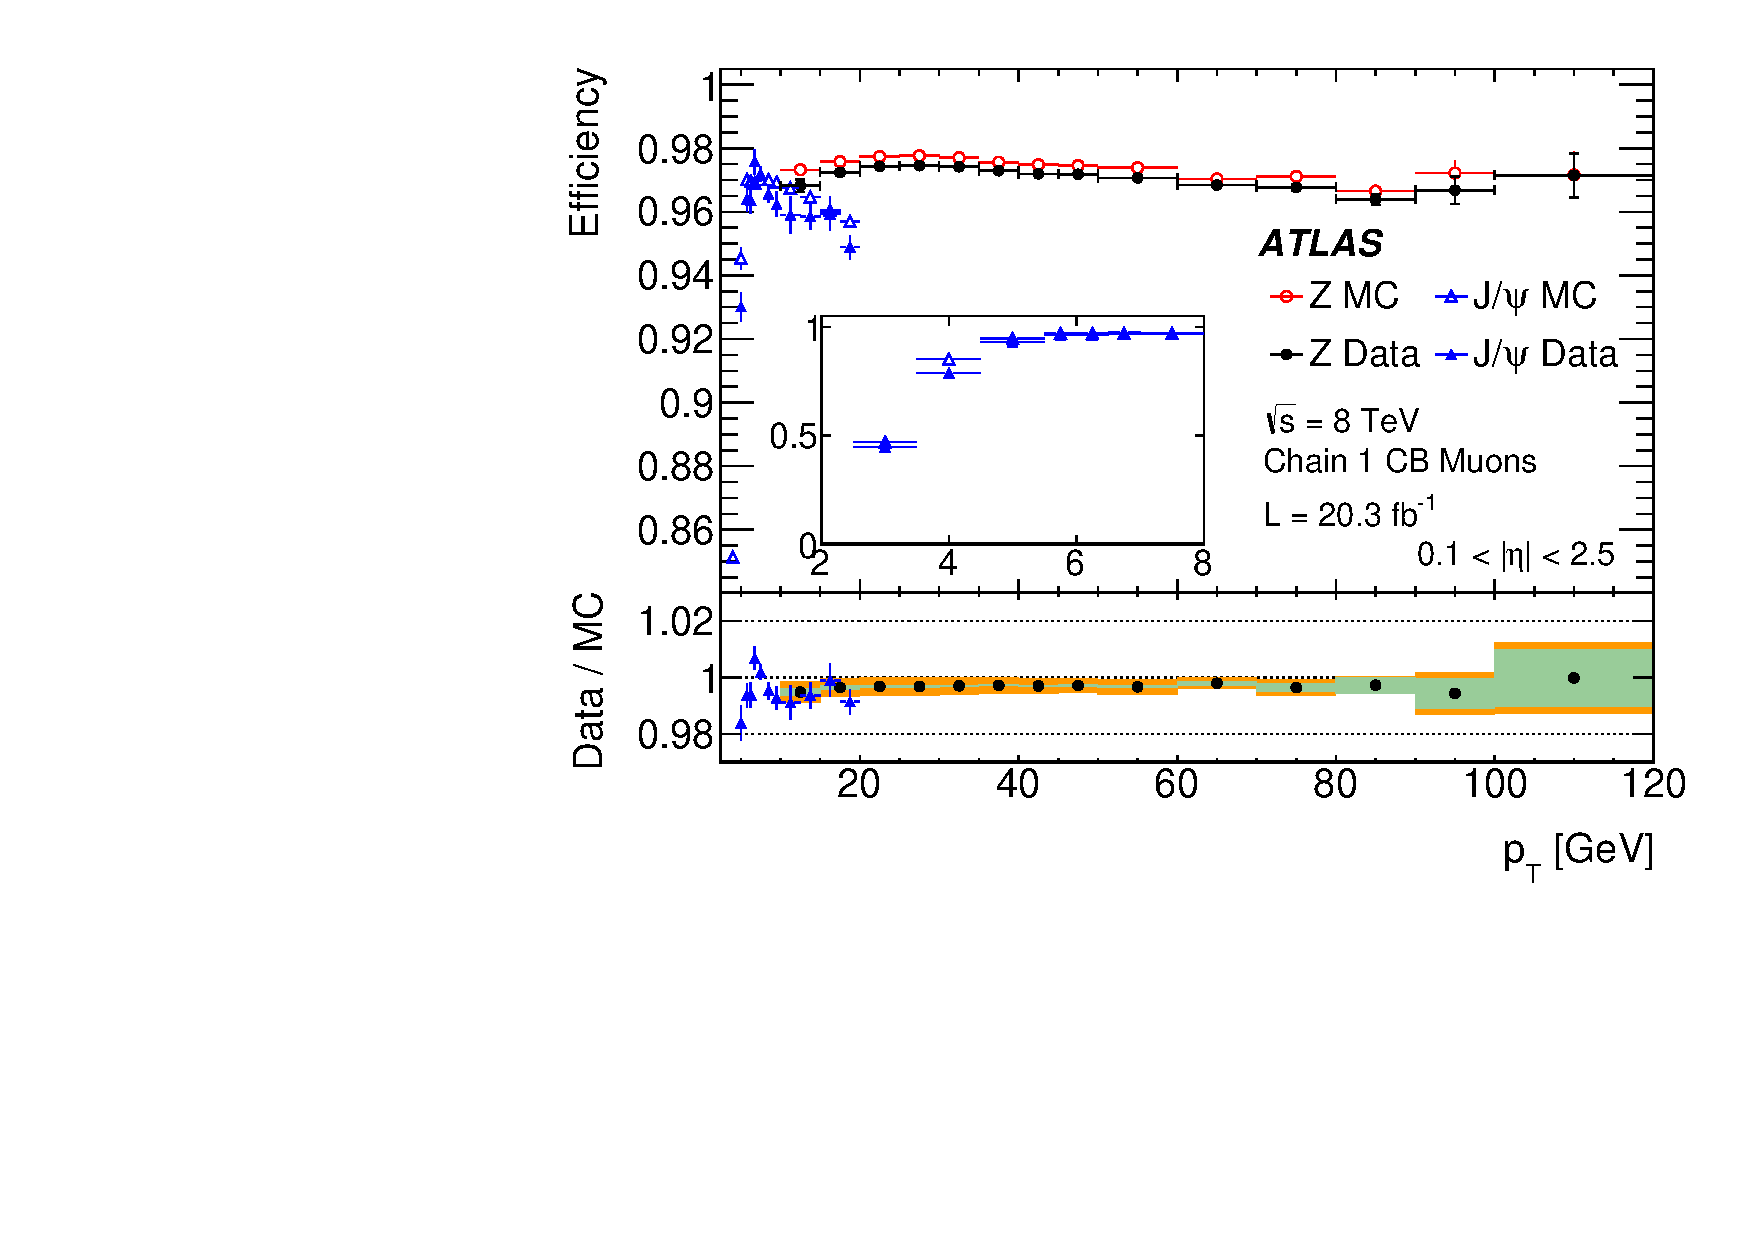
\includegraphics[width=0.4\textwidth]{fig/reconstruction/muon_TP_pt.pdf}
    \label{chap:reconstruction:fig:muon_tp_pt}
    }
    \caption[]{Muon identification efficiency as a function of
      $\eta$ for the different muon
      types~\subref{chap:reconstruction:fig:muon_tp_eta}, and as a
      function of \pt~for CB muons~\subref{chap:reconstruction:fig:muon_tp_pt}~\cite{bib:Aad:2014rra}.}
\label{chap:reconstruction:fig:muon_tp}
\end{figure}

As for electrons, the ratio of the efficiency measured in data to
simulation is computed. In order to recover the correct reconstruction
and identification efficiencies in simulation, these scale factors are
applied to all predictions from MC in two-dimensional $\eta-\phi$
bins. In addition to efficiency corrections, the muon momentum scale
and resolution is corrected in simulation, with corrections that are
determined in a likelihood fit to data. Scale corrections are less
than 0.1\% in most $\eta$ regions, and as high as 0.4\% in the region
$1.25 < \eta < 1.5$. Muon resolution is corrected in MC by applying a
``smearing'' term to the reconstructed \pt. This smearing correction is
less than 10\% for the ID and less than 15\% for the MS. Systematic
uncertainties on these corrections will be discussed in section~\ref{}.
